\newpage
\section{Result}

In \autoref{fig:result_figure} one can see the given spectrum together with gaussian fits of all the peaks. The extracted mean peak angle, the standard deviation and the calculated full with maxima (using \autoref{eq:FWHM}) can bee seen in \autoref{tab:sample1} and \autoref{tab:sample2}. 

\begin{figure}[H]
    \centering
    \begin{subfigure}[b]{0.89\textwidth} 
        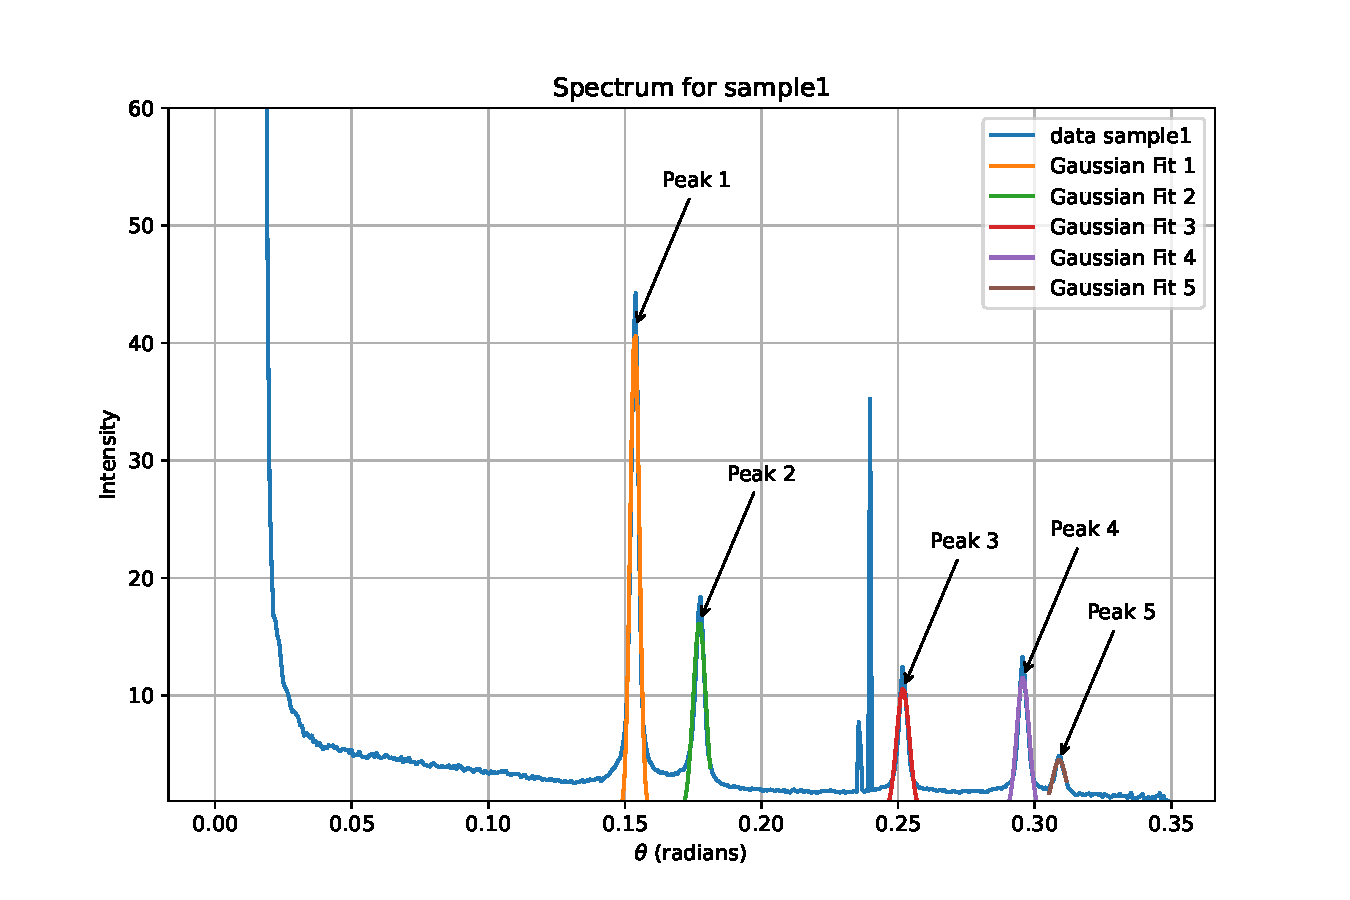
\includegraphics[width=\textwidth]{Figures/gaussian_sample1.pdf}
        \subcaption{This is the first subfigure.}
        \label{fig:subfigure1}
    \end{subfigure}
    \begin{subfigure}[b]{0.89\textwidth} 
        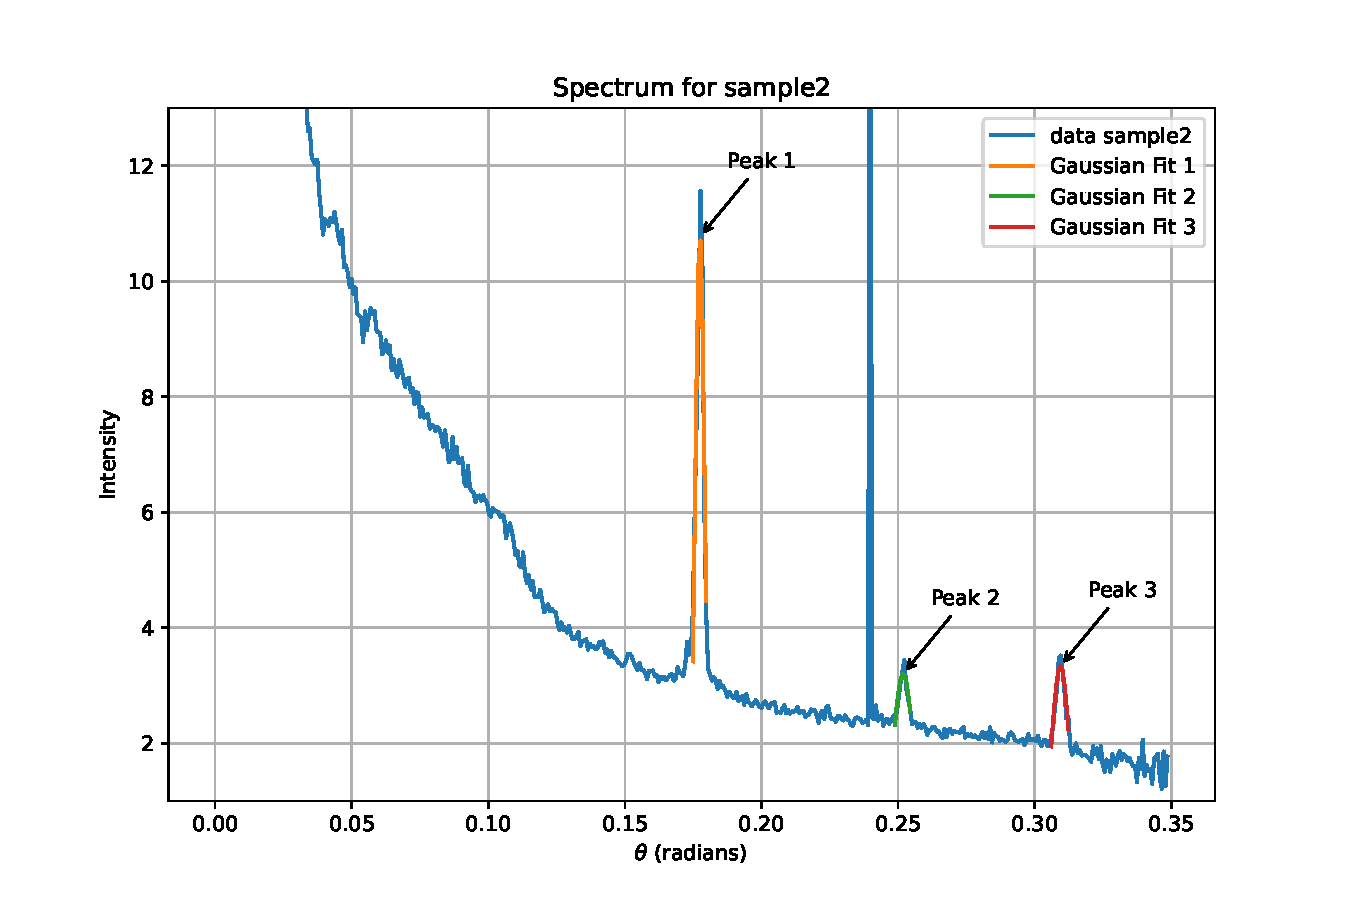
\includegraphics[width=\textwidth]{Figures/gaussian_sample2.pdf}
        \subcaption{This is the second subfigure.}
        \label{fig:subfigure2}
    \end{subfigure}
    \caption{This figure shows two subfigures with separate captions.}
    \label{fig:result_figure}
\end{figure}

\begin{table}[H]
    \centering
    \caption{Fitting results for Sample 1}
    \begin{tabular}{cccc}
    \toprule
    Peak & Angle $\theta$ (radians) & Standard deviation $\sigma$ (radians) & FWHM (radians) \\
    \midrule
    Peak 1 & \num{0.15362(0.00010)}{} & \num{0.00165(0.00010)} & \num{0.00388(0.00023)}{} \\
    Peak 2 & \num{0.17731(0.00019)}{} & \num{0.00227(0.00020)}{} & \num{0.00535(0.00046)}{} \\
    Peak 3 & \num{0.25180(0.00018)}{} & \num{0.00234(0.00018)}{} & \num{0.00550(0.00043)}{} \\
    Peak 4 & \num{0.29569(0.00015)}{} & \num{0.00225(0.00015)}{} & \num{0.00530(0.00035)}{} \\
    Peak 5 & \num{0.30900(0.00015)}{} & \num{0.00261(0.00021)}{} & \num{0.00616(0.00049)}{} \\
    \bottomrule
    \end{tabular}
    \label{tab:sample1}
\end{table}

\begin{table}[H]
    \centering
    \caption{Fitting results for Sample 2}
    \begin{tabular}{cccc}
    \toprule
    Peak & Angle $\theta$ (radians) & Standard deviation $\sigma$ (radians) & FWHM (radians) \\
    \midrule
    Peak 1 & \num{0.17746(0.00012)}{} & \num{0.00172(0.00014)}{} & \num{0.00404(0.00034)}{} \\
    Peak 2 & \num{0.25186(0.00017)}{} & \num{0.00380(0.00039)}{} & \num{0.00895(0.00092)}{} \\
    Peak 3 & \num{0.30942(0.00014)}{} & \num{0.00326(0.00024)}{} & \num{0.00768(0.00056)}{} \\
    \bottomrule
    \end{tabular}
    \label{tab:sample2}
\end{table}

Using peak 1 from the first sample and $n=1$, the plane (111) we obtain a spacing $a=\SI{4.0213(0.0026)}{\angstrom}$ which coincides with the material Au using \autoref{eq:Bragg} and \autoref{eq:seperation} with the given table \cite{solidstatephysics2025}. The first peak coincides with the plane (111) as seen in \autoref{eq:ordering} and all indices are odd which is must be true since Au is a fcc. This verifies this result. 

Using peak 2 from the second sample and $n=1$, the plane (110) we obtain a spacing $a=\SI{2.8484(0.0030)}{\angstrom}$ which coincides with the material Fe using \autoref{eq:Bragg} and \autoref{eq:seperation} with the given table \cite{solidstatephysics2025}. The second peak coincides with the plane (110) as seen in \autoref{eq:ordering}, also the sum of the miller indices is even which must be tru for a bcc such as Fe, verifying this result. 


Using \autoref{eq:Scherre}, we obtain the following particle sizes as shown in \autoref{tab:Scherre1} and \autoref{tab:Scherre2}. The mean particle size for Sample 1 is \SI[scientific-notation=false]{13.44(0.4)}{\nano\meter}, and for Sample 2, it is \SI[scientific-notation=false]{11.2(0.6)}{\nano\meter}.


\begin{table}[H]
    \centering
    \begin{minipage}{0.45\textwidth}
        \centering
        \caption{Powder size $t$ for Sample 1}
        \begin{tabular}{cc}
        \toprule
        Peak & Size (\SI{}{\m}) \\
        \midrule
        Peak 1 & \num{17.4(10)e-8} \\
        Peak 2 & \num{12.7(11)e-8} \\
        Peak 3 & \num{12.5(10)e-8} \\
        Peak 4 & \num{13.2(9)e-8} \\
        Peak 5 & \num{11.4(9)e-8} \\
        \bottomrule
        \end{tabular}
        \label{tab:Scherre1}
    \end{minipage}%
    \hfill
    \begin{minipage}{0.45\textwidth}
        \centering
        \caption{Powder size $t$ for Sample 2}
        \begin{tabular}{cc}
        \toprule
        Peak & Size (\SI{}{\m}) \\
        \midrule
        Peak 1 & \num{1.68(14)e-8} \\
        Peak 2 & \num{7.7(8)e-9} \\
        Peak 3 & \num{9.1(7)e-9} \\
        \bottomrule
        \end{tabular}
        \label{tab:Scherre2}
    \end{minipage}
\end{table}